%\documentclass[aps,prb, twocolumn, 10pt]{revtex4-2}
\documentclass[aps,prb, 10pt]{revtex4-2}

\usepackage{amssymb,amsmath}
\usepackage{graphicx}
\usepackage{natbib}
\usepackage{multirow}

\usepackage{lipsum}

\usepackage[utf8]{inputenc}

\begin{document}

\title{Theoretical modeling of the collective tunneling of a Wigner necklace}

\author{D. Szombathy$^1$, M. A. Werner$^{1, 2}$, P. C. Moca$^{1, 3}$, I. Shahal$^{4}$, A. Hamo$^{4}$ and G. Zaránd $^{1,2}$}
\affiliation{$^1$Department of Theoretical Physics, Institute of Physics, Budapest University of Technology and Economics, Műegyetem rkp. 3., H-1111 Budapest, Hungary\\ $^2$MTA-BME Quantum Dynamics and Correlations Research Group,
Budapest University of Technology and Economics, Műegyetem rkp. 3., H-1111 Budapest, Hungary\\ $^3$Department of Theoretical Physics, University of Oradea, 410087, Oradea, Romania\\ $^4$}


\begin{abstract}
	% WCCT main latex files abstract
\lipsum[1]
\end{abstract}

\maketitle

\begin{figure}[h]
\centering
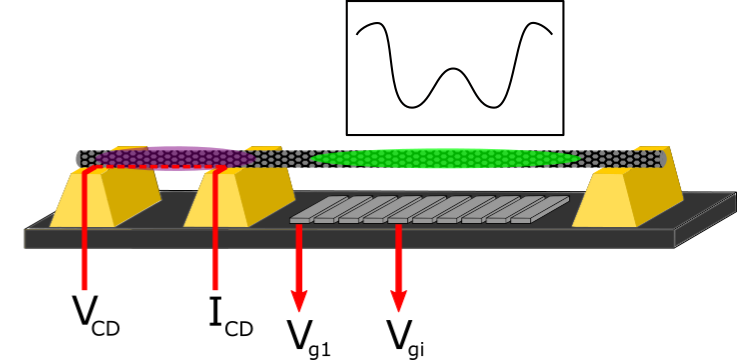
\includegraphics[width=1\textwidth]{Experimental Setup}
\label{ExperimentalSetup}
\caption{Experimental setup scematics}
\end{figure}

\begin{figure}[h]
\centering
\includegraphics[width=1\textwidth]{1stimage}
\label{1stImage}
\caption{Effective potential in case of 3 particles and wavefunction density as a function of detuning paramtere ($\epsilon$)}
\end{figure}

\begin{figure}[h]
\centering
\includegraphics[width=1\textwidth]{Polarizationcomparison}
\label{2ndImage}
\caption{Polarization as a function of detuning, compraed to experiment}
\end{figure}



\end{document}